Arbeidspunktet ligger midt på lastlinja.
Altså i det aktive området.
\\
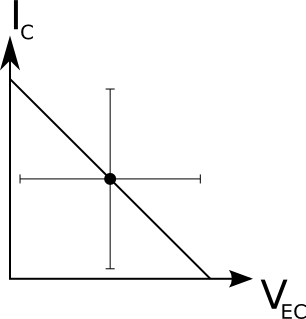
\includegraphics[width=0.5\textwidth]{./img/typeALastlinje}
\\\\
Effektforsterker klasse A (emitterfølger)
\\
\begin{circuitikz} \draw
(4,2) node[npn] (npn) {}
      (npn.base) node[anchor=east] {}
      (npn.collector) node[anchor=south] {}
      (npn.emitter) node[anchor=north] {}

(0,2) node[label=$V_{inn}$] {}
      to[C, o-] (2,2)
      -- (npn.base)
(2,2) to[R, l=$R_1$] (2,4)
      -- (4,4)
      -- (npn.collector)
(2,2) to[R, l=$R_2$] (2,-1)
(npn.emitter) to[R, l=$R_E$] (4,-1)
(4,1) to[short, -o] (6,1)
      node[label=$V_{ut}$] {}
(4,-1) -- (0,-1)
      node[ground] {}
      ;
\end{circuitikz}
\\\\
TypeA effektforsterkere har lav virkningsgrad. f.eks $\eta = 25\%$.
Denne klassen trekker strøm når det ikke er tilført signal.
